% ****** Start of file .tex ******
%
%   This file is based on apssamp.tex, part of the APS files in the REVTeX 4.1 distribution.
%   Version 4.1r of REVTeX, August 2010
%
%   Copyright (c) 2009, 2010 The American Physical Society.
%   Samuel Balula, Pedro Ribeiro, Luís Macedo, Eduardo Neto 2013
%   See the REVTeX 4 README file for restrictions and more information.
%
% TeX'ing this file requires that you have AMS-LaTeX 2.0 installed
% as well as the rest of the prerequisites for REVTeX 4.1
%
% See the REVTeX 4 README file
% It also requires running BibTeX. The commands are as follows:
%
%  1)  latex filename.tex
%  2)  bibtex filename
%  3)  latex filename.tex
%  4)  latex filename.tex

\documentclass[%
  reprint,
  %superscriptaddress,
  %groupedaddress,
  %unsortedaddress,
  %runinaddress,
  %frontmatterverbose, 
  %preprint,
  %showpacs,preprintnumbers,
  nofootinbib,
  %nobibnotes,
  %bibnotes,
  amsmath,amssymb,
  aps,
  %pra,
  %prb,
  %rmp,
  %prstab,
  %prstper,
  %floatfix,
  10pt,
  a4paper
]{revtex4-1}



\usepackage{facil}                      % Pacote pessoal
\usepackage{verbatim}                   % Apresentação de código
\usepackage{graphicx}                   % Include figure files
\usepackage{dcolumn}                    % Align table columns on decimal point
\usepackage{bm}                         % bold math
\usepackage[latin1,utf8]{inputenc}      % Tipos de caracteres
\usepackage[portuges]{babel}            % Português
\usepackage{indentfirst}                % Identação da primeira linha
\usepackage{hyperref}                   % add hypertext capabilities
\usepackage{float}                      %Fixar imagens
%\usepackage[mathlines]{lineno}          % Enable numbering of text and display math
%\linenumbers\relax                      % Commence numbering lines
%\usepackage[compact]{titlesec}

\usepackage[%showframe,%Uncomment any one of the following lines to test 
%%scale=0.7, marginratio={1:1, 2:3}, ignoreall, % default settings
%%text={7in,10in},centering,
margin=0.5in,        %diminuir margens
%total={6.5in,8.75in}, top=1.2in, left=0.9in, 
includefoot
%height=10in,a5paper,hmargin={3cm,0.8in},
]{geometry}

\begin{document}
\preprint{APS/123-QED}
%\captionsetup[table]{font=small,skip=0pt}
%\captionsetup[figure]{font=small,skip=0pt}
%\titlespacing{\section}{0pt}{*0}{*0}            %Poupar espaço
%\titlespacing{\subsection}{0pt}{*0}{*0}
%\titlespacing{\subsubsection}{0pt}{*0}{*0}


% % % % % % % % % % % % % % % % % % % % % % % % % % % % % % % % % % % % % % % % 
%%%%%%%%%%%%%%%%%%%%%%%%%%%%%%%%%% Início %%%%%%%%%%%%%%%%%%%%%%%%%%%%%%%%%%%%%%
% % % % % % % % % % % % % % % % % % % % % % % % % % % % % % % % % % % % % % % %
 

\title{Levitação magnética com electroiman e fotoresistência}
%\thanks{}

\author{Pedro Ribeiro}%
\email{73221, pedro.q.ribeiro@tecnico.ulisboa.pt}
\author{Luis Macedo}%
\email{73633, luis.macedo@tecnico.ulisboa.pt}
\author{Samuel Balula}%
\email{72735, samuel.balula@tecnico.ulisboa.pt}

\affiliation{
  Instituto Superior Técnico\\
  Mestrado em Engenharia Física Tecnológica\\
  Complementos de Electrónica
}

%\collaboration{Grupo 57}

\date{\today}

%%%%%%%%%%%%%%%%%%%%%%%%%%%%%%%%%% Abstract %%%%%%%%%%%%%%%%%%%%%%%%%%%%%%%%%%%%
\begin{abstract}
Neste trabalho laboratorial implementa-se um sistema de controlo que mantém em levitação um objeto metálico não magnetizado. Para tal utilizou-se um electroíman e uma fotoresistência e implementou-se um circuito que se encarregou do controlo do sistema. Conseguiu-se manter o objecto em levitação, contudo o sistema era muito instável e quando ocorria uma perturbação o equilibrio era perdido.
%1


\end{abstract}
\maketitle


%%%%%%%%%%%%%%%%%%%%%%%%%%%%%%%%%% Introdução %%%%%%%%%%%%%%%%%%%%%%%%%%%%%%%%%%
\section{Introdução}
\label{s:intro}
%Situar o problema, incluir fórmulas.
%Quem lê o relatório deve conseguir perceber exatamente o que foi feito.
%2

O objectivo deste trabalho é implementar um circuito que faça o controlo de um sistema com o objectivo de manter em levitação um objecto metálico não magnetizado. Pretende-se que o circuito controle a corrente que passa nas bobines que criam o campo magnético que produz a força magnética no objecto, que o faz levitar. O circuito que faz o controlo é constituido por vários andares sendo que estes serão explicados na secção \ref{s:expreal}. Um dos conceitos importantes no que toca a controlo de sistemas é o PID (proporcional, integral e diferencial). Neste caso não se implementou a parte da diferenciação, pois apesar de ajudar no resultado pretendido, não seria suficiente para melhorar em termos consideráveis os resultados, uma vez que o objecto metálico era colocado na posição pretendida manualmente, ou seja, a resposta do circuito para tempos muito pequenos não precisava de ser melhorada ao ponto de se implementar um circuito diferenciador. Implementou-se assim a parte do integrador que tinha como função que o objecto metálico se mantivesse na posição pretendida.


%%%%%%%%%%%%%%%%%%%%%%%%%%%% Experiência realizada %%%%%%%%%%%%%%%%%%%%%%%%%%%%%
\section{Experiência Realizada}
\label{s:expreal}
%Incluir diagrama de blocos da montagem
De acordo com as instruções do guia, implentou-se o circuito da \rfig{../img/esquematico.png}. Apresentam-se na tabela \ref{partlist} os componentes eléctricos utilizados, montados numa breadboard.

%\figurao{../img/esquematico.png}{Circuito implementado no laboratório}



\tabela[partlist]{Lista dos componentes utilizados}{lrrr}{
	Descrição		&Modelo/Valor		&Qt.			&Referência	\\ \hline
	Bobine c/ núcleo ferro	&			&1			&L1		\\
	Fotoresistência		&			&1			&R3		\\
	Trans. J. Bipolar NPN	&2N3055			&1			&Q1		\\
	Trans. J. Bipolar PNP	&MJ2955			&1			&Q2		\\
	Ampl. operacional	&LM741			&5			&UX		\\
	LED			&red			&1			&LED		\\
	Cond. electrolítico	&1$\mu$F		&1			&C1		\\
	Potenciómetro		&10K$\Omega$		&1			&R5		\\
	Resistência .25W	&100$\Omega$		&1			&R0		\\
	Resistência .25W	&300$\Omega$		&1			&R4		\\
	Resistência .25W	&1K$\Omega$		&1			&R10		\\
	Resistência .25W	&2.2K$\Omega$		&1			&R12		\\
	Resistência .25W	&5.6K$\Omega$		&1			&R1		\\
	Resistência .25W	&10K$\Omega$		&1			&R2		\\
	Resistência .25W	&15K$\Omega$		&1			&R11		\\
	Resistência .25W	&56K$\Omega$		&4			&R6-9		\\
	%3
}

Para facilidade de análise, divide-se o circuito nas suas partes constituintes, que se analisam separadamente.


\subsection{LED}
%4
\fig[.2]{../img/led.png}{Circuito do LED}

Para iluminar um led, colocado em frente à fotoresistência, utilizou-se o circuito da \rfig{../img/led.png}. Para a tensão de alimentação de cerca de 10V utilizada, a corrente é dada por \eqref{eled}. O valor é suficientemente alto para que a intensidade da radiação emitida influence a resistência variável fotosensível, estando dentro dos limites eléctricos de funcionamento.

\eq[eled]{I=\frac{V_{cc}-V_d}{R_0} \approx 93 mA}
	
	
\subsection{Divisor de Tensão}
%Da a tensao de referencia
%5

\fig{../img/divtensao.png}{Excerto do esquemático representando o divisor de tensão}

O circuito apresentado na \rfig{../img/divtensao.png} é um simples divisor de tensão, formado pelas resistências R1 e R2, e um seguidor de tensão, em que se usa um amplificador operacional LM741. Para uma tensão de referência de 10V, obtÊm-se uma referência de 3.6V. Utiliza-se este divisor afim de evitar tensões (e correntes) excessivas nos andares seguintes, em particular tendo em conta a fotoresistência, que pode apresentar resistências da ordem das centenas de $\Omega$.






\subsection{Fotoresistência}
%6
Uma fotoresistência é um componente composto por um material que sofre variação da sua resistividade com a variação da intensidade da luz incidente neste (também conhecido como fotocondutividade).\\
O dispositivo utilizado sofria um aumento da sua condutividade (e consequentemente uma diminuição da resistência) com o aumento da intensidade luminosa. Integrando este dispositivo num divisor de tensão, como se mostra na figura \ref{fig:foto_res}, que obedece à relação:
\begin{equation}
V_{out}=\frac{R_3}{R_3+R_4}V_{in}
\label{eq:div_t}
\end{equation}
\begin{figure}[h]
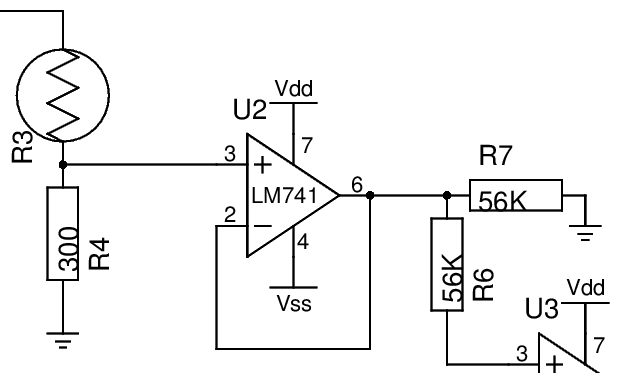
\includegraphics[width=3in]{../img/sensor.png}
\caption{Esquemático do divisor de tensão de tensão onde se inseriu o sensor ($R_3$) com seguidor de tensão.}
\label{fig:foto_res}
\end{figure}
Desta forma, e de acordo com a relação obtida em \ref{eq:div_t}, o sinal de saída do divisor de tensão será tanto maior quanto maior for a resistência $R_3$, ou seja, quanto menor for a intensidade da luz incidente no sensor.\\
Coloca-se um seguidor de tensão em série com a saída do divisor de tensão para minimizar a impedância de saída deste.


\subsection{Tensão de referência}
%7
De modo a definir uma tensão de referência com a qual trabalhar e para ser de fácil ajuste utilizou-se um potenciómetro. Esta parte do circuito encontra-se representada na figura \ref{fig:tensaoreferencia}, sendo que o potenciómetro é representado pela resistência $R_5$. Esta tensão de referência liga posteriormente ao somador integrador. É de salientar que é esta tensão de referência que vai determinar qual a distância que queremos entre o objecto metálico e o electroíman.

\begin{figure}[h]
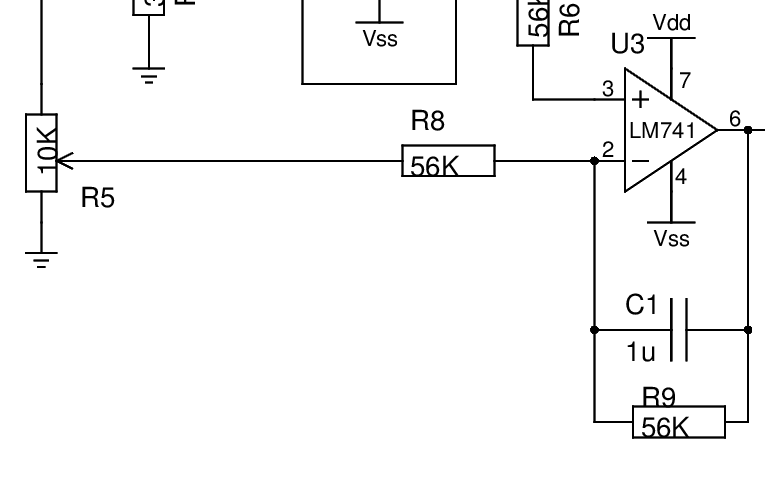
\includegraphics[width=3in]{../img/ref.png}
\caption{Esquemático do potenciómetro utilizado, que é representado pela resistência $R_5$.}
\label{fig:tensaoreferencia}
\end{figure}




\subsection{Somador integrador}
%8
O somador integrador utilizado pode ser decomposto como sendo um somador e um integrador em série, como está representado no esquema da figura \ref{fig:intg}.
\begin{figure}[h]
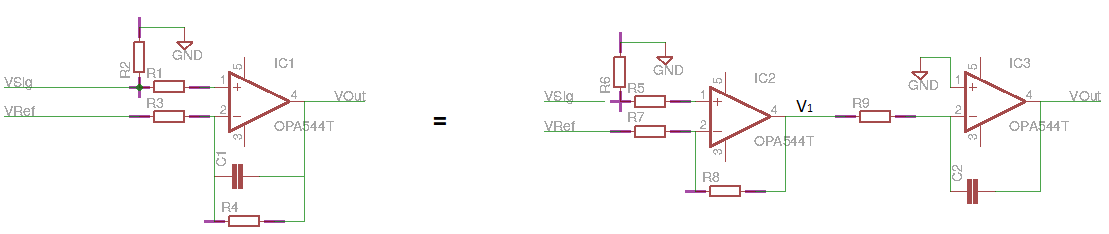
\includegraphics[width=3in]{../img/intg.png}
\caption{Esquemático do somador integrador utilizado e do esquema equivalente.}
\label{fig:intg}
\end{figure}
Assim, para calcular qual o valor de tensão à saída deste bloco, primeiro será necessário calcular qual a tensão à saída do somador e de seguida, qual a tensão à saída do integrador.\\
Assumindo que as resistências são todas iguais (como é o caso na montagem utilizada) com valor $R$, utlizando a lei da sobreposição, tem-se que, anulando $V_{Ref}$:
\begin{equation}
\frac{V_{Sig}}{R}=\frac{V_1-V_{in}}{R}\Rightarrow V_1=2V_{Sig}
\end{equation}
Por outro lado, anulando $V_{Sig}$:
\begin{equation}
\frac{V_{ref}}{R}=-\frac{V_1}{R}\Rightarrow V_{1}=-V_{Ref}
\end{equation}
Somando as duas contribuições é possível obter o valor de tensão à entrada do bloco integrador:
\begin{equation}
V_1=2V_{Sig}-V_{Ref}
\end{equation}
Para o bloco integrador, a equação que descreve o circuito é simplesmente:
\begin{equation}
C\frac{\mathrm{d}V_{out}}{\mathrm{d}t}=-\frac{V_1}{R}
\end{equation}
O que resulta em (resolvendo a equação diferencial):
\begin{equation}
V_{out}(t)=V_1(t=0)- \frac{ 1 }{RC} \int_{0}^{T}V_{\text{1}}(t)\, \operatorname{d}t
\end{equation}
E consequentemente:
\begin{equation}
V_{out}(t)=-\frac{ 1 }{RC} \int_{0}^{T}2V_{Sig}(t)-V_{Ref}(t)\, \operatorname{d}t
\end{equation}
Visto que a resistência utilizada tinha $R=56\mathrm{k}\Omega$ e o condensador $C=1\mu$F, a constante de tempo deste integrador é $\tau=RC=56\mathrm{ms}$.
A função do somador integrador é adicionar inércia ao sistema, isto é, fazer com que os valores de saída tenham tendência a ir de forma menos impulsiva para o valor de referência (que aconteceria caso só houvesse bloco proporcional ou diferencial neste PID).
\subsection{Amplificador não inversor}
%9

Considere-se a tipologia apresentada na \rfig{../img/somador1.png}.

\fig{../img/somador1.png}{Circuito somador}
\fig{../img/somador2.png}{Circuito somador genérico}

\eq{V_0=V_+ - R_r i_{R_r}}
\eq{\frac{V_3-V_+}{R_3}+\frac{V_4-V_+}{R_4}=i_{R_r}}
\eq{V_0=V_+-R_r\lr{\frac{V_3-V_+}{R_3} + \frac{V_4-V_+}{R_4}}}

\eq{0 = \frac{V_1-V_+}{R_1} + \frac{V_2-V_+}{R_2}}
\eq{V_+=\frac{\frac{V_1}{R_1} + \frac{V_2}{R_2}}{\frac{1}{R_1} + \frac{1}{R_2}}}

Generalizando para j entradas não inversoras e k entradas inversoras, de acordo com o esquema da \rfig{../img/somador2.png}
\eq[sum1]{V_+ = \frac{\sum_{i=1}^{j}{\frac{V_{pi}}{R_{pi}}}}{\sum_{i=1}^{j}{\frac{1}{R_{pi}}}}}
\eq[sum2]{V_0 = V_+ - R_r \sum_{i=1}^{k}{\frac{V_{mi}-V_+}{R_{mi}}}}

Tomando $V_{p1}=V_{in}$, $R_{p1}=0$, $V_{m1}=0$, $R_{m1}=R10$ e $R_r = R_{11}$, \eqref{sum1} e \eqref{sum2} tomam a forma:
\eq{V_+ = V_{in}}
\eq{V_0 = V_+\lr{1+\frac{R_{11}}{R_{10}}}}

Isto é, um amplificador não inversor. Para os valores das resistências utilizadas têm-se um factor de ganho 16.








\subsection{Rectificação}
%10
Implementou-se no circuito um rectificador, sendo que a função deste é fazer com que o objecto metálico não magnetizado não seja atraído quando está demasiado perto do electroíman. Isto é conseguido uma vez que quando o objecto está mais próximo do electroíman do que se pretende (distância definida com a tensão de referência) o sinal produzido é negativo, e o objecto continuaria a ser atraído. Contudo com a implementação do rectificador isto já não acontece. Este rectificador está representado na figura \ref{fig:rectificador}.
\begin{figure}[h]
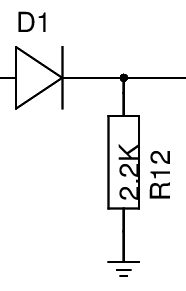
\includegraphics[width=1.5in]{../img/rectificador.png}
\caption{Esquemático rectificador implementado.}
\label{fig:rectificador}
\end{figure}





\subsection{Andar de saída em classe B}
%11
O andar de saída utilizado nesta montagem (e representado na figura \ref{fig:B_team}) para alimentar a bobina que servia de electroíman, foi um andar em classe B, visto que este andar possui boa eficiência, um ganho de corrente elevado, pois este é dado por:
\begin{equation}
i_o=(\beta_f+1)i_i
\end{equation}
Onde $\beta_f\approx70$ e principalmente, porque o atraso entre a chegada do sinal a amplificar na entrada e a emissão do sinal amplificado na saída era muito reduzido. É de notar também que para o aparelho a controlar, a distorção de cruzamento era desprezável.
\begin{figure}[h]
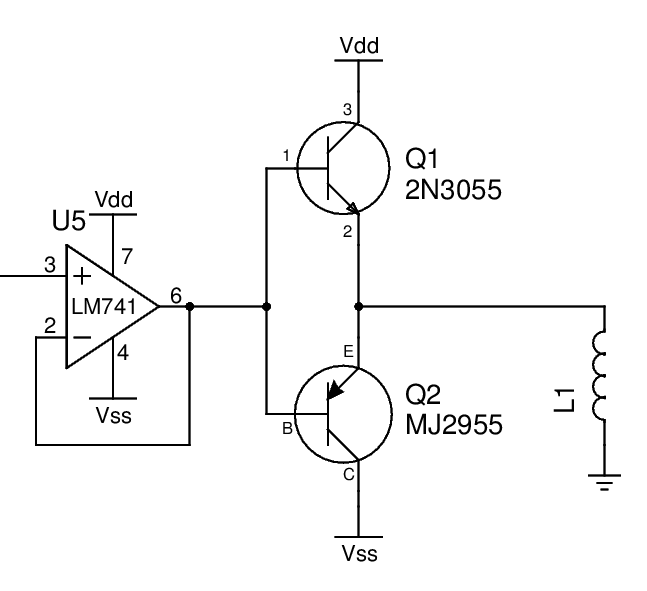
\includegraphics[width=3in]{../img/andardesaida.png}
\caption{Esquemático do andar de saída em classe B implementado.}
\label{fig:B_team}
\end{figure}
Realça-se que o sinal de entrada foi condicionado de maneira a que os transístores do andar de saída nunca entrassem na zona de saturação.


%%%%%%%%%%%%%%%%%%%%%%%%%%%%%%%% Resultados %%%%%%%%%%%%%%%%%%%%%%%%%%%%%%%%%%%%
\section{Resultados}
\label{s:resul}
%incluir tabelas. Excesso de dados => grafico com valores mais significativos
%12
Com o circuito utilizado, observou-se que o objecto metálico era incapaz de levitar e em vez disso, quando estava no ponto mais afastado da bobina o campo magnético induzido era máximo e o objecto subia até ao ponto máximo (onde está mais próximo da bobina) e quando atingia essa posição, o campo magnético induzido seria nulo e o objecto metálico voltaria a descer até a posição mais afastada da bobina por acção da gravidade.\\
Isto significa que em vez de se obter o comportamento esperado, que seria a levitação magnética do objecto numa posição fixa, obteve-se um movimento oscilatório do objecto metálico.\\
É de notar que, numa ocasião, foi possível colocar o objecto a levitar, colocando-o manualmente na posição de equilíbrio deste sistema. No entanto apurou-se que este equílibrio não era estável, pois uma pequena vibração da mesa ou um pequeno impacto no aparelho faziam com que o objecto metálico voltasse a oscilar novamente.\\




%%%%%%%%%%%%%%%%%%%%%%%%%%% Conclusões e Críticas %%%%%%%%%%%%%%%%%%%%%%%%%%%%%%
\section{Conclusões e Críticas}
\label{s:conclu}
%Incluir melhorias propostas à experiência
Foi possível colocar o objecto em levitação, apesar de este se encontrar num equilíbrio instável que era facilmente perturbável. Uma das razões pelas quais não se conseguiu obter um resultado mais estável foi devido à magnetização induzida no objecto, que permanecia nele instantes após a anulação do campo magnético. Isto fazia com o objecto em vez de deixar de sentir a força magnética, continuasse a ser atraído em direcção à bobine durante alguns instantes, perturbando assim o sistema.\\
Uma solução testada para tentar resolver este problema, foi a utilização de um magneto, um objecto metálico com um momento magnético permanente, que permitiria utilizar o campo magnético da bobina tanto para repelir como para atrair o magneto (algo que não é possível com o objecto metálico não magnetizado). No entanto, esta solução provou ser pouco eficaz, visto que é necessário uma grande precisão na quantidade de corrente que percorre a bobina, pois até uma pequena variação do campo magnético gerado provocava grande força a atuar no magneto (o que tornou o sistema mais instável).\\
Uma sugestão para conseguir um maior equílibrio do sistema seria adicionar atrito ao sistema, de modo que a força magnética não induzisse movimentos tão impulsivos no objecto metálico, dando assim mais tempo ao sistema para reagir atempadamente às perturbações.





%\begin{acknowledgments}
%\end{acknowledgments}

%%%%%%%%%%%%%%%%%%%%%%%%%%%%%%%%%%%%%%%%%%%%%%%%%%%%%%%%%%%%%%%%%%%%%%%%%%%%%%%%
% % % % % % % % % % % % % % % %     FIM    % % % % % % % % % % % % % % % % % % % 
%%%%%%%%%%%%%%%%%%%%%%%%%%%%%%%%%%%%%%%%%%%%%%%%%%%%%%%%%%%%%%%%%%%%%%%%%%%%%%%%

\nocite{*}
\bibliography{bibliografia}{}
\bibliographystyle{plain}% Produces the bibliography via BibTeX.
\end{document}
%end of file
